\chapter{Fondre et bouillir~: les changements d'état}\label{ch:g4:changes-of-state}

Tu sais depuis des années que la chaleur fait \omterm{def:g2:ice-water-steam:meltfreeze}{fondre} la glace et
bouillir l'eau. Mais tu possèdes maintenant un \omterm{def:g3:temperature-thermometers:temperature}{thermomètre} --- et le
\omterm{def:g3:temperature-thermometers:temperature}{thermomètre} a quelque chose d'étonnant à rapporter du fond du seau de
glace qui fond~: pendant que la glace fond, la \omterm{def:g3:temperature-thermometers:temperature}{température}
\emph{refuse de bouger}. Regardons les vieux changements d'état avec
des yeux neufs.

\section{Les noms savants}

Les changements d'état de l'eau reçoivent maintenant leurs noms de
grands, valables pour toutes les matières et pas seulement pour
l'eau. Du \omterm{def:g3:solids-liquids-gases:solid}{solide} au \omterm{def:g3:solids-liquids-gases:liquid}{liquide}~: la \emph{fusion}\index{fusion}. Du
\omterm{def:g3:solids-liquids-gases:liquid}{liquide} au \omterm{def:g3:solids-liquids-gases:solid}{solide}~: la \emph{solidification}\index{solidification}
(on dit aussi congélation). Du \omterm{def:g3:solids-liquids-gases:liquid}{liquide} au \omterm{def:g3:solids-liquids-gases:gas}{gaz}~:
l'\emph{ébullition}\index{ébullition} quand cela se produit vite,
avec de grosses bulles, et l'évaporation quand cela se produit
tranquillement à la surface. Du \omterm{def:g3:solids-liquids-gases:gas}{gaz} au \omterm{def:g3:solids-liquids-gases:liquid}{liquide}~: la condensation.
Toutes les matières du monde --- l'eau, le chocolat, le fer, l'or ---
peuvent jouer à ce jeu, chacune à ses propres \omterm{def:g3:temperature-thermometers:temperature}{températures}.

\begin{definition}[Température de fusion]\label{def:g4:changes-of-state:melting-point}
La \emph{température de fusion}\index{température de fusion} d'une
matière est la \omterm{def:g3:temperature-thermometers:temperature}{température} à laquelle elle fond --- et aussi celle à
laquelle le \omterm{def:g3:solids-liquids-gases:liquid}{liquide} se solidifie de nouveau. Pour l'eau, elle vaut
\qty{0}{\celsius}. Chaque matière a la sienne~: le chocolat fond vers
\qty{34}{\celsius} (la \omterm{def:g3:temperature-thermometers:temperature}{température} de la bouche --- ce n'est pas un
hasard, demande à un chocolatier), la cire de bougie vers
\qty{60}{\celsius}, le fer seulement à \qty{1538}{\celsius}.
\end{definition}

\begin{definition}[Température d'ébullition]\label{def:g4:changes-of-state:boiling-point}
La \emph{température d'ébullition}\index{température d'ébullition}
d'une matière est la \omterm{def:g3:temperature-thermometers:temperature}{température} à laquelle elle bout. Pour l'eau,
elle vaut \qty{100}{\celsius}. Là encore, chaque matière a la
sienne --- c'est pourquoi un cuisinier attentif peut faire s'\omterm{def:g2:ice-water-steam:evapcond}{évaporer}
toute l'eau pendant que l'huile de la même poêle reste
tranquillement \omterm{def:g3:solids-liquids-gases:liquid}{liquide}.
\end{definition}

\begin{example}[Lire le monde avec deux
nombres]\label{ex:g4:changes-of-state:reading}
Pourquoi une tablette de chocolat est-elle \omterm{def:g3:solids-liquids-gases:solid}{solide} sur l'étagère
(\qty{20}{\celsius}) mais \omterm{def:g3:solids-liquids-gases:liquid}{liquide} dans ta poche lors d'une randonnée
d'été (\qty{35}{\celsius})~? Parce que sa \omterm{def:g4:changes-of-state:melting-point}{température de fusion},
proche de \qty{34}{\celsius}, se trouve \emph{entre} les deux. Une
matière est \omterm{def:g3:solids-liquids-gases:solid}{solide} au-dessous de sa \omterm{def:g4:changes-of-state:melting-point}{température de fusion}, \omterm{def:g3:solids-liquids-gases:liquid}{liquide}
au-dessus --- et cela jusqu'à sa \omterm{def:g4:changes-of-state:boiling-point}{température d'ébullition}, où elle
s'en va sous forme de \omterm{def:g3:solids-liquids-gases:gas}{gaz}. Deux nombres racontent toute l'histoire
d'une matière à n'importe quelle \omterm{def:g3:temperature-thermometers:temperature}{température}.
\end{example}

\section{Le thermomètre têtu}

\begin{method}[Regarder fondre la glace comme il
faut]\label{met:g4:changes-of-state:watch}
\begin{enumerate}
  \item Remplir un saladier de glace pilée ou de neige et y planter
        le \omterm{def:g3:temperature-thermometers:temperature}{thermomètre}~; attendre et lire~: \qty{0}{\celsius}~;
  \item apporter le saladier dans la cuisine chaude et lire le
        \omterm{def:g3:temperature-thermometers:temperature}{thermomètre} toutes les quelques minutes pendant que la glace
        fond~;
  \item continuer à lire longtemps après la disparition du dernier
        éclat de glace.
\end{enumerate}
Le rapport~: pendant toute la fusion --- eau et glace ensemble dans
le saladier --- le \omterm{def:g3:temperature-thermometers:temperature}{thermomètre} reste obstinément à \qty{0}{\celsius}.
Ce n'est que lorsque le \emph{dernier} morceau de glace a fondu que
la \omterm{def:g3:temperature-thermometers:temperature}{température} se met à monter.
\end{method}

\begin{proposition}[La loi du palier]\label{prop:g4:changes-of-state:plateau}
Pendant qu'une matière change d'état --- qu'elle fond ou qu'elle
bout --- sa \omterm{def:g3:temperature-thermometers:temperature}{température} reste immobile au repère, quel que soit le
travail de la cuisinière. Toute la chaleur qui arrive est dépensée
pour le changement d'état lui-même, et rien pour monter. Le \omterm{def:g3:solids-liquids-gases:solid}{solide} et
le \omterm{def:g3:solids-liquids-gases:liquid}{liquide} cohabitent à la \omterm{def:g4:changes-of-state:melting-point}{température de fusion}~; le \omterm{def:g3:solids-liquids-gases:liquid}{liquide} et le
\omterm{def:g3:solids-liquids-gases:gas}{gaz}, à la \omterm{def:g4:changes-of-state:boiling-point}{température d'ébullition}.
\end{proposition}

\begin{omfigure}
\begin{tikzpicture}
\begin{axis}[omaxis, width=10.5cm, height=5.6cm,
    xlabel={temps sur la cuisinière}, ylabel={température (\unit{\celsius})},
    xtick=\empty, ytick={0,100},
    ymin=-40, ymax=140, xmin=0, xmax=10]
  \addplot[very thick, omDef] coordinates
    {(0,-30) (1.5,0) (3.5,0) (5.5,100) (8.5,100)};
  \addplot[very thick, omThm] coordinates {(8.5,100) (9.6,132)};
  \node[below, font=\small] at (axis cs:2.5,-4) {la glace fond~: palier};
  \node[above, font=\small] at (axis cs:7.0,103) {l'eau bout~: palier};
\end{axis}
\end{tikzpicture}

{\small Une casserole de glace sur une cuisinière régulière, racontée
par le \omterm{def:g3:temperature-thermometers:temperature}{thermomètre}~: la \omterm{def:g3:temperature-thermometers:temperature}{température} monte, s'arrête à
\qty{0}{\celsius} pendant que la glace fond, remonte, et s'arrête à
\qty{100}{\celsius} pendant que l'eau s'en va en bouillant. (La
dernière montée rouge appartient à la vapeur.)}
\end{omfigure}

\begin{omfigure}
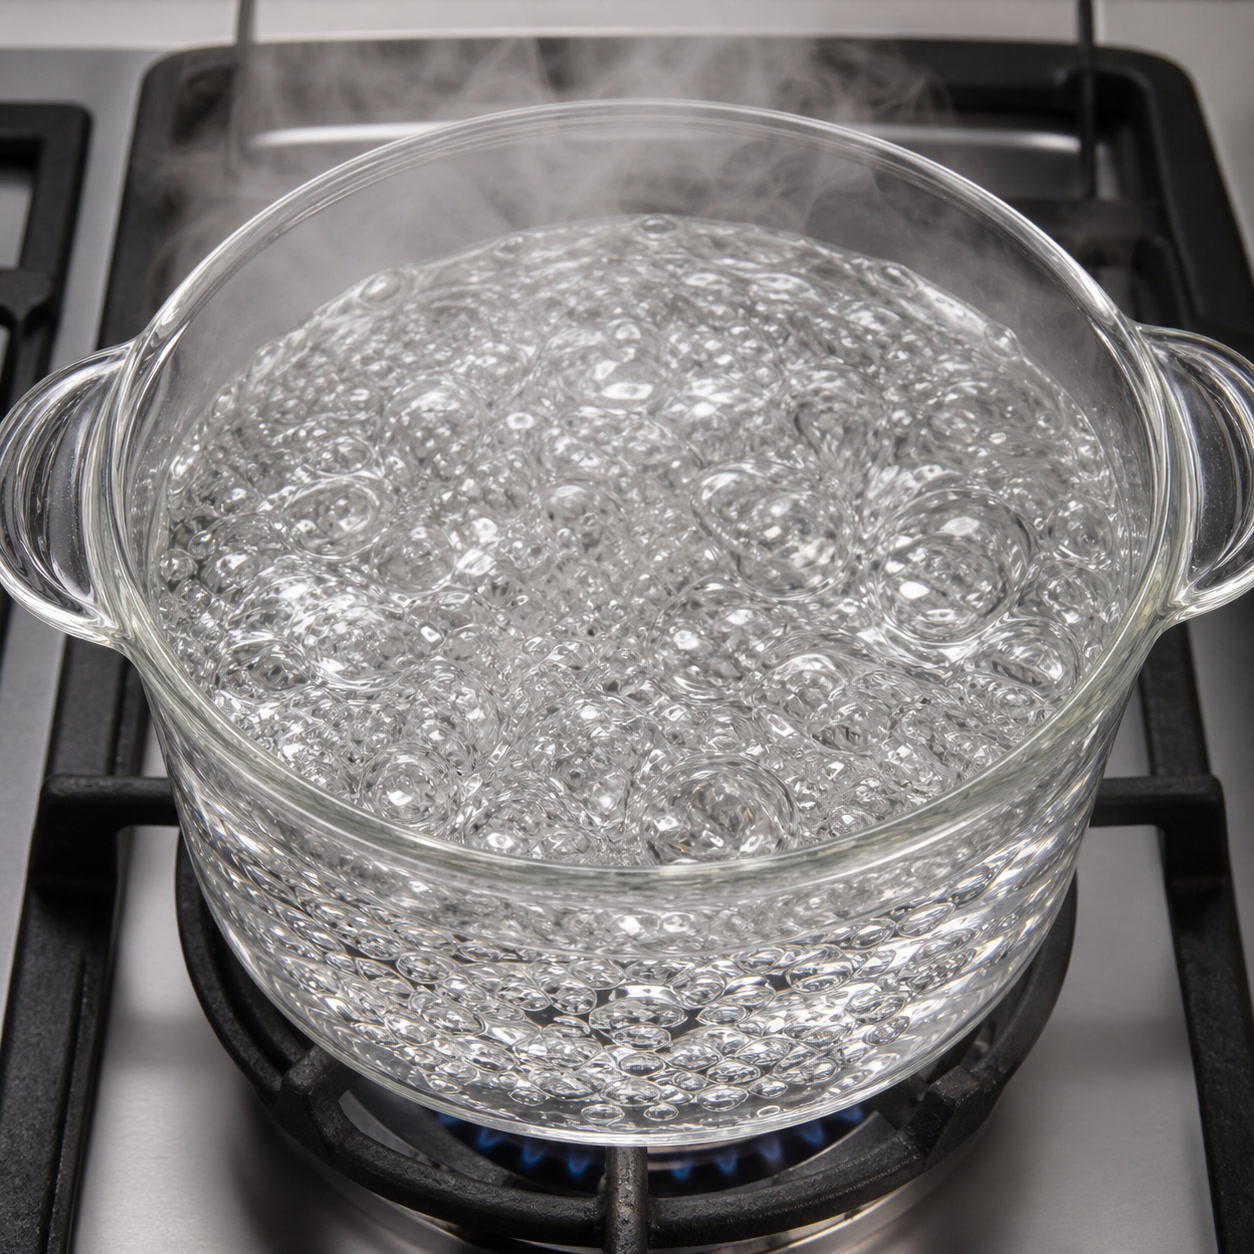
\includegraphics[width=0.45\linewidth]{images/book1/ai/g4-changes-boiling-pot.jpg}

{\small Un bouillonnement à gros bouillons~: des bulles de vapeur d'eau se forment dans le \omterm{def:g3:solids-liquids-gases:liquid}{liquide} et éclatent à la surface --- et pendant tout ce temps, le \omterm{def:g3:temperature-thermometers:temperature}{thermomètre} reste immobile à la \omterm{def:g4:changes-of-state:boiling-point}{température d'ébullition}.}
\end{omfigure}

\begin{example}[Le palier dans la cuisine]\label{ex:g4:changes-of-state:kitchen}
Voilà pourquoi une eau qui frémit et une eau qui bout à gros
bouillons cuisent les pâtes aussi vite~: les deux casseroles sont
exactement à \qty{100}{\celsius} --- la seconde ne fait que gaspiller
sa chaleur supplémentaire en fabriquant de la vapeur plus vite. Et
voilà pourquoi une boisson avec des glaçons reste à \qty{0}{\celsius}
jusqu'au dernier éclat de glace~: la glace qui fond cloue la
\omterm{def:g3:temperature-thermometers:temperature}{température} au repère.
\end{example}

\begin{remark}[Un nombre que l'œil ne peut pas
voir]\label{rem:g4:changes-of-state:invisible}
Sans \omterm{def:g3:temperature-thermometers:temperature}{thermomètre}, personne ne devinerait le palier~: la casserole
semble de plus en plus agitée, le seau de glace de plus en plus
calme, et dans les deux la \omterm{def:g3:temperature-thermometers:temperature}{température} ne bouge pas d'un pouce. C'est
une victoire de plus de la mesure sur l'apparence --- et l'une des
premières grandes surprises que les instruments aient jamais offertes
à la science.
\end{remark}

\section{Chaque matière garde ses repères}

\begin{proposition}[Les repères sont des marques
d'identité]\label{prop:g4:changes-of-state:identity}
La \omterm{def:g4:changes-of-state:melting-point}{température de fusion} et la \omterm{def:g4:changes-of-state:boiling-point}{température d'ébullition} d'une matière
pure ne changent jamais~: l'eau fond à \qty{0}{\celsius} aujourd'hui,
demain, dans un palais ou sous une tente. Ces repères font partie de
l'identité de la matière --- si bien gardés qu'un scientifique peut
reconnaître une matière inconnue en mesurant où elle fond et où elle
bout.
\end{proposition}

\begin{example}[La bougie et la fonderie]\label{ex:g4:changes-of-state:foundry}
Une bougie près de la cheminée s'affaisse et \omterm{def:g1:floating-and-sinking:words}{coule}~: la cire a
dépassé sa \omterm{def:g4:changes-of-state:melting-point}{température de fusion}, proche de \qty{60}{\celsius}. Dans
une fonderie, des ouvriers versent du fer \omterm{def:g3:solids-liquids-gases:liquid}{liquide} orange
incandescent comme de la soupe --- leur four a dépassé
\qty{1538}{\celsius}. Même jeu, repères follement différents~: ce que
la cheminée fait à la cire, seul un four peut le faire au fer. Et
l'or fond à \qty{1064}{\celsius}~: les orfèvres connaissent ce
nombre, dans leurs mains sinon en degrés, depuis des milliers
d'années.
\end{example}

\begin{omfigure}
\begin{tikzpicture}[scale=0.85]
  \draw[-Stealth, very thick] (0.5,0) -- (11.2,0);
  \node[right, font=\small] at (11.15,0.4) {plus chaud};
  \foreach \x/\t/\name in {1.3/0/{la glace fond}, 3.1/34/{chocolat},
      4.4/60/{cire}, 6.2/100/{l'eau bout}, 8.3/1064/{or},
      10.1/1538/{fer}} {
    \draw[thick] (\x,-0.12) -- (\x,0.12);
    \node[above, font=\footnotesize] at (\x,0.2) {$\t$};
    \node[below, font=\footnotesize, align=center] at (\x,-0.2) {\name};
  }
\end{tikzpicture}

{\small Les repères de quelques matières de tous les jours, en \omterm{def:g3:temperature-thermometers:temperature}{degrés
Celsius} (la droite est comprimée --- le repère du fer se trouve
vraiment quinze fois plus loin que celui de l'eau). Chaque matière
porte ses propres nombres, toujours.}
\end{omfigure}

\section{Exercices}

\begin{exercise}[$\star$]\label{exo:g4:changes-of-state:1}
Donne le nom savant~: du \omterm{def:g3:solids-liquids-gases:solid}{solide} au \omterm{def:g3:solids-liquids-gases:liquid}{liquide}~; \ du \omterm{def:g3:solids-liquids-gases:liquid}{liquide} au
\omterm{def:g3:solids-liquids-gases:solid}{solide}~; \ du \omterm{def:g3:solids-liquids-gases:liquid}{liquide} au \omterm{def:g3:solids-liquids-gases:gas}{gaz} avec de grosses bulles~; \ du \omterm{def:g3:solids-liquids-gases:gas}{gaz} au
\omterm{def:g3:solids-liquids-gases:liquid}{liquide} sur une vitre froide.
\end{exercise}

\begin{exercise}[$\star$]\label{exo:g4:changes-of-state:2}
Quels sont les deux repères de l'eau, avec leurs \omterm{def:g3:temperature-thermometers:temperature}{températures}~? Et
celle de la fusion du chocolat, à peu près~?
\end{exercise}

\begin{exercise}[$\star$]\label{exo:g4:changes-of-state:3}
Un saladier contient de la glace et de l'eau ensemble, bien
mélangées. Qu'indique le \omterm{def:g3:temperature-thermometers:temperature}{thermomètre}~? Qu'indiquera-t-il cinq minutes
plus tard, s'il reste encore de la glace~?
\end{exercise}

\begin{exercise}[$\star$]\label{exo:g4:changes-of-state:4}
Énonce la loi du palier. Où passe la chaleur de la cuisinière pendant
que l'eau bout, puisque la \omterm{def:g3:temperature-thermometers:temperature}{température} ne monte plus~?
\end{exercise}

\begin{exercise}[$\star$]\label{exo:g4:changes-of-state:5}
La cire fond vers \qty{60}{\celsius}. Une bougie est-elle \omterm{def:g3:solids-liquids-gases:solid}{solide} ou
\omterm{def:g3:solids-liquids-gases:liquid}{liquide}~: dans un salon à \qty{20}{\celsius}~? \ à côté d'une flamme
qui la chauffe à \qty{80}{\celsius}~? \ dans un grenier d'été à
\qty{35}{\celsius}~?
\end{exercise}

\begin{exercise}[$\star$]\label{exo:g4:changes-of-state:6}
Les pâtes cuisent dans une eau qui bout doucement. Papa met le feu au
maximum et la casserole bout à gros bouillons. L'eau est-elle plus
chaude maintenant~? Que produit la chaleur supplémentaire à la
place~?
\end{exercise}

\begin{exercise}[$\star$]\label{exo:g4:changes-of-state:7}
Sur le graphique du palier de ce chapitre, comment repérer les deux
changements d'état sans lire un seul mot~?
\end{exercise}

\begin{exercise}[$\star$]\label{exo:g4:changes-of-state:8}
Le fer fond à \qty{1538}{\celsius} et l'or à \qty{1064}{\celsius}. Un
four fonctionne à \qty{1200}{\celsius}~: lequel des deux métaux y
\omterm{def:g1:floating-and-sinking:words}{coule} comme de la soupe, et lequel reste \omterm{def:g3:solids-liquids-gases:solid}{solide}~? De combien de
degrés le four manque-t-il l'autre~?
\end{exercise}

\begin{exercise}[$\star$]\label{exo:g4:changes-of-state:9}
Pourquoi une boisson avec des glaçons reste-t-elle aussi froide
jusqu'au dernier éclat de glace --- et ne commence-t-elle à se
réchauffer qu'ensuite~?
\end{exercise}

\begin{exercise}[$\star\star$]\label{exo:g4:changes-of-state:10}
Une scientifique reçoit un \omterm{def:g3:solids-liquids-gases:solid}{solide} blanc inconnu. Elle trouve qu'il
fond exactement à \qty{0}{\celsius} et que son \omterm{def:g3:solids-liquids-gases:liquid}{liquide} bout
exactement à \qty{100}{\celsius}. Quelle est sa meilleure hypothèse
sur cette matière --- et quelle loi permet aux repères de servir de
carte d'identité~?
\end{exercise}

\begin{exercise}[$\star\star$]\label{exo:g4:changes-of-state:11}
Des alpinistes racontent que, très haut sur les grands sommets, l'eau
bout alors qu'elle est \emph{tout juste} trop chaude pour qu'on y
touche --- et que leur thé n'infuse jamais correctement. Quelle
certitude de tous les jours sur l'eau qui bout s'effondre là-haut~?
(La raison se cache dans l'\omterm{def:g2:air-around-us:air}{air} lui-même, et un chapitre plus loin sur
la pression de l'\omterm{def:g2:air-around-us:air}{air} la débusquera.)
\end{exercise}
